\documentclass[a4paper,12pt]{article}
\usepackage{ctex}
\usepackage{geometry}
\usepackage{amsmath}
\usepackage{amssymb}
\usepackage{amsthm}
\usepackage{graphicx}
\usepackage{listings}
\usepackage{booktabs}
\usepackage{float}
\usepackage{color}


\geometry{left=2cm, right=2cm, top=2cm, bottom=2cm}

% 用来设置附录中代码的样式

\lstset{
    basicstyle          =   \sffamily,          % 基本代码风格
    keywordstyle        =   \bfseries,          % 关键字风格
    commentstyle        =   \rmfamily\itshape,  % 注释的风格,斜体
    stringstyle         =   \ttfamily,  % 字符串风格
    flexiblecolumns,                % 别问为什么,加上这个
    numbers             =   left,   % 行号的位置在左边
    showspaces          =   false,  % 是否显示空格,显示了有点乱,所以不现实了
    numberstyle         =   \zihao{-5}\ttfamily,    % 行号的样式,小五号,tt等宽字体
    showstringspaces    =   false,
    captionpos          =   t,      % 这段代码的名字所呈现的位置,t指的是top上面
    frame               =   lrtb,   % 显示边框
}

\lstdefinestyle{Python}{
    language        =   Python, % 语言选Python
    basicstyle      =   \zihao{-5}\ttfamily,
    numberstyle     =   \zihao{-5}\ttfamily,
    keywordstyle    =   \color{blue},
    keywordstyle    =   [2] \color{teal},
    stringstyle     =   \color{magenta},
    commentstyle    =   \color{red}\ttfamily,
    breaklines      =   true,   % 自动换行,建议不要写太长的行
    columns         =   fixed,  % 如果不加这一句,字间距就不固定,很丑,必须加
    basewidth       =   0.5em,
}

\lstdefinestyle{html}{
    language        =   html, % 语言选Python
    basicstyle      =   \zihao{-5}\ttfamily,
    numberstyle     =   \zihao{-5}\ttfamily,
    keywordstyle    =   \color{blue},
    keywordstyle    =   [2] \color{teal},
    stringstyle     =   \color{magenta},
    commentstyle    =   \color{red}\ttfamily,
    breaklines      =   true,   % 自动换行,建议不要写太长的行
    columns         =   fixed,  % 如果不加这一句,字间距就不固定,很丑,必须加
    basewidth       =   0.5em,
}



\title{基于Lucene和Bootstrap的耳机检索网站的构建}
\author{ICE2602 Group 2}

\begin{document}
    \maketitle

    \begin{abstract}
        对于本次大作业,我们小组选择了题目2,并将关注点聚焦到耳机这一商品上。通过爬取京东、苏宁易购以及亚马逊上的耳机产品,我们实现了基本的搜索功能。进一步地,我们结合不同框架实现了前端页面的设计与美化,并实现了以下功能:

        \begin{itemize}
            \item 采集了来自京东、苏宁易购、亚马逊商城的共计10603条有效产品数据,并建立了搜索索引,实现了基本搜索功能
            \item 能根据商品名称、商品属性、关键词、商品图片的描述文字进行检索,并将结果通过前端进行反馈。
            \item 以前端交互的方式按相关度、价格等属性进行排序,并将结果进行反馈。
            \item 以前端交互的方式按类别、品牌、特性等属性进行过滤,并将结果通过前端反馈。
            \item 能基于商品的评论数进行排序,并将结果通过前端反馈。
            \item 能实现基于品牌名称和logo图像的搜索,并将结果通过前端反馈。
        \end{itemize}
    \end{abstract}

    \newpage

    \tableofcontents

    \newpage

    \section{引言}

    目前,人们的生活已经离不开电商平台所提供的种种服务,而搜索功能则作为其中最为基本、核心的功能。在课堂的学习中,我们了解了搜索引擎工作的基本原理,索引的构建以及搜索功能的实现,以及诸如PageRank等经典算法的实现。在本次大作业中,我们旨在利用自己本学期所学习的内容将搜索引擎的知识进行结合,同时利用一定的图像分析基础来实现更加进阶的功能。

    在本次大作业中,我们的许多功能设计参考了京东网上商城的排版以及UI设计。图\ref{fig:1}展示了京东网页版的搜索界面,在这里我们选取“耳机”作为关键词。从中我们可以看出,在主要搜索栏中包含了品牌的筛选、佩戴方式(也即耳机功能)的筛选、连接方式的筛选等。同时,商品可以按照“综合”、“销量”、“评论数”、“价格”等关键属性进行排序。而在商品的展示阶段,则采用了网格式设计,以图片和其价格作为核心,辅以商品名称和其它辅助信息。

    \begin{figure}[H]
        \centering
        \includegraphics[scale=0.3]{pic/pic1.png}
        \caption{京东商城搜索“耳机”所得到的搜索结果}
        \label{fig:1}
    \end{figure}

    为了实现这一功能,我们小组将任务进行了拆解并进行了合理的分工,具体如下:
    \begin{itemize}
        \item 核心信息的搜集、索引文件的构建(裴圣鑫)。数据是搜索引擎中最为基本、最为核心的要素。由于我们需要对2-3个电商平台进行网页的爬取,因而统一数据类型以及数据整理这一工作变得十分关键。
        \item 基于Flask框架的前后端互联以及搜索功能的初步实现(郭润泽)。后端的索引建立完成之后,需要通过相应的python框架来实现用户在前端输入以及后台的交互功能,也即将原本在控制台上运行的种种命令转移到前端进行。
        \item 基于BootStrap的前端设计和页面美化(朱鹏翔)。在网页的基本框架和核心搜索功能完成之后,核心任务便是完成过滤、筛选等一系列更加精细化的操作。这些操作同样要求对前后端交互的实现进行较为充分的把握。
        \item 基于神经网络的图片搜索(周晟洋)。在上述基于文本的搜索功能实现之后,我们还可以利用下半学期所学的图像处理的相关知识将图片进行识别并转化为关键词,依次来扩大搜索的范围,进一步完善网站的功能。
    \end{itemize}

    \section{基于网络爬虫的数据收集与整理}

    \section{基于Lucene的搜索引擎核心算法构建}


    \section{基于BootStrap的前端设计和页面美化}

    \subsection{前端设计引言}

    前端即网站前台部分,运行在PC端,移动端等浏览器上展现给用户浏览的网页。随着互联网技术的发展,HTML5,CSS3,前端框架的应用,跨平台响应式网页设计能够适应各种屏幕分辨率,合适的动效设计,给用户带来极高的用户体验。在搜索引擎的构建过程中,前端是其中必不可少的部分,作为沟通爬取数据和搜索界面的桥梁,我们使用课程中学习的Flask进行网页搜索和前端的基础,同时建立html文件对搜索网页进行美化和排版等构建,便于用户搜索和操作。

    \subsection{Flask实现前后端的交互}

    主函数中的Flask函数的构造和之前所学习的Lab构造方法一样,同样是由一个form函数生成搜索的区域用于在html文件中通过action进行对接,另一个函数对应着搜索之后跳转的网页页面,同样返回用户所需要了解的对应信息,两个网页风格保持一致,其中Flask在主函数中的代码体现如下:

    \begin{lstlisting}[language=python]
    web = Flask(__name__)
    @web.route('/form', methods=['POST', 'GET'])
    def bio_data_form():
    if request.method == "POST":
        keyword = request.form['keyword']
        
        return redirect(url_for('result', keyword=keyword))
    return render_template("index.html")

    @web.route('/result', methods=['GET', 'POST'])
    def result():
        STORE_DIR = "index"
        vm_env.attachCurrentThread()
        directory = SimpleFSDirectory(File(STORE_DIR).toPath())
        searcher = IndexSearcher(DirectoryReader.open(directory))
        analyzer = SimpleAnalyzer()
        keyword = request.args.get('keyword')
        keyword = ' '.join(jieba.cut(keyword))
    \end{lstlisting}

    % 由于此处实现与Lab 7中较为类似,因而我们并不做过多的阐述,只列举两个较为典型的问题
    % \begin{itemize}
    %     \item 关于VMinit()函数——启动Java虚拟机是使用lucene的必要步骤,但在Flask的框架上应该要求在发送第一个request之前就完成这个操作,这要求构建一个装饰器@app.before_first_request,并且在原先的搜索文件中加入以下两行代码
    %     \begin{lstlisting}[language=python]
    % vm_env = lucene.getVMEnv()
    % vm_env.attachCurrentThread()
    %     \end{lstlisting}
    %     注意这两行代码需要添加在所有用到lucene库中Index、Search等函数的最前面
    %     \item 针对Flask框架下html网页中对列表信息的提取建议用字典形式的数据,其格式为each.key而非python语法中的each[key]。如果使用正常的循环写法,则需要特别注意i的大小和数据之间的对应关系。
    % \end{itemize}

    \subsection{前端框架的确立与网页的基本搭建}

    在前端的开发与页面布局时, HTML将元素进行定义,CSS对展示的元素进行定位,再通过JavaScript实现相应的效果和交互。为了能够以较为美观的方式来展示页面,我们利用了Bootstrap这一经典组件库来辅助网页的构建。Bootstrap是美国Twitter公司的设计师Mark Otto和Jacob Thornton合作基于HTML、CSS、JavaScript所开发的简洁、直观、强悍的前端开发框架,使得Web开发更加快捷。Bootstrap提供了优雅的HTML和CSS规范,它即是由动态CSS语言Less写成。在本次大作业中,我们使用了最新版本的Bootstrap 5.0来进行。在本次作业中,我们采用了\textbf{动态导入}的方法,因而在程序运行时需要保证网络的畅通,并且存在由于Bootstrap服务器连接出现问题而使得网页渲染不成功的情况,在测试时需要特别注意。

    首先我们需要实现的是主页的设计,我们采取简约使用风格的进行构图,因此在各个组件的颜色和背景上并没有过多的渲染。以简单的黑白蓝三色作为网页的基本色调,整体结构则是由网页的top,section,bottom这三部分组成,top和bottom均按照Bootstrap所提供的navbar模板分别对应着标题和结尾。基于上述框架所设计的主页如图\ref{fig:13}所示,整体而言较为美观。在网页上侧布置了基于文本搜索和后续基于图片搜索的额两种搜索框,我们还添加了常用链接来填充页面,使得整体结构较为美观,所对应的核心HTML代码附在下方。

    \begin{figure}[H]
        \centering
        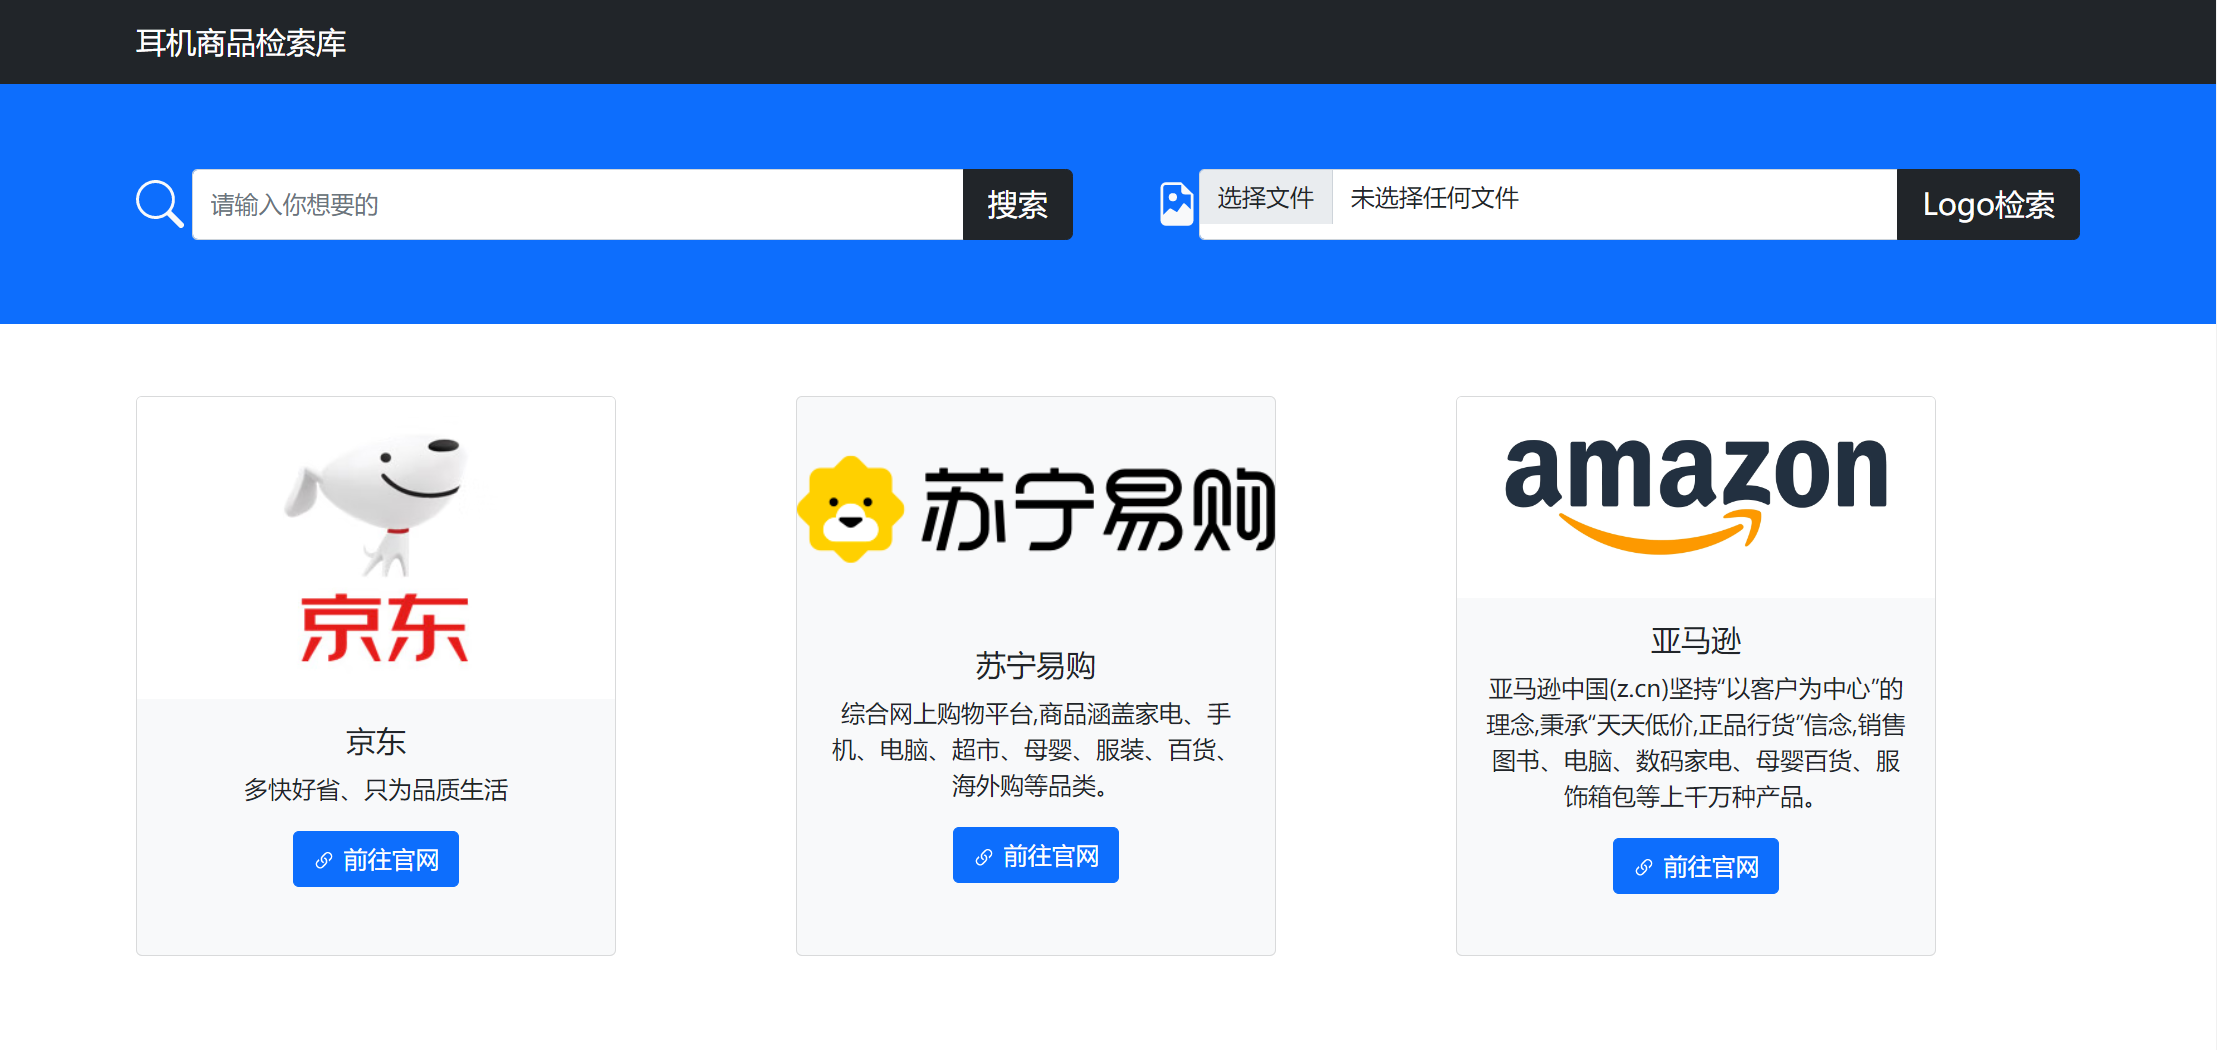
\includegraphics[scale=0.4]{pic/pic13.png}
        \caption{搜索主页的设计}
        \label{fig:13}
    \end{figure}

    \begin{lstlisting}[language=html]
    <nav class="navbar navbar-expand-lg bg-dark navbar-dark fixed-top">
        <div class="container">
            <a href="#" class="navbar-brand">Online Shopping</a>
            <button class="navbar-toggler" 
            type="button" data-bs-toggle="collapse" data-bs-target="#navmenu">
                <span class="navbar-toggler-icon"></span>
            </button>
        </div>
    </nav>
    \end{lstlisting}

    对于主体部分,我们采用分块的section进行构造,主体大致可以分为简介,搜索部分和推荐网站部分,搜索部分则是其中重点,此区块和前面的主函数部分连接,通过已经学习过的Flask实现。在进行这一部分的处理时,考虑到商品搜索之后需要给用户呈现出的内容较多,我们相应的设置了很多相关变量进行传参,例如商品名称简介和链接,店铺名称和链接,对应的图片和链接,还有诸如评价和价格等相关信息,对于排版我们致力于做到简洁明了,使用户得到最好的体验。

    而实现此区块我们使用了Bootstrap中的Card组件,这样可以将大面积的网页区块化,使得呈现出来的信息条理清晰。而基于各大网购网页的分析我们知道,搜索呈现的结果必定是按照矩阵排列的,所以我们对于此section的处理也是如此,在其中加入row,col参数将Card按照搜索先后排列出来,在此区域的处理中,遇到的难点是对于整体的搜索结果而言总量为多少未知,而横行Card数量设置为3,所以当搜索出来的条目非3的倍数时,会出现Card为空的现象,对于此处,我们则采用固定的搜索结果进行限制,将其按照搜索先后即重要程度进行取舍,以保证呈现出来的结果完整。在HTML代码的撰写中,我们同样基于所学的Flask框架语法来设计循环结构,核心结构如下

    \begin{lstlisting}[language=html]
    
    <div class="col-md">
    <div class="card bg-light text-dark" style="width: 20rem;">
        <div class="card-body text-center">
            <div class="card-text">
                {{title_lst[3*i-3]}}
            </div>
            <img src="{{pic_url_lst[3*i-3]}}
            " alt="" class="w-50 done d-md-center mt-4">
            <div class="row my-5">
                <a href="{{shop_url_lst[3*i-3]}}
            " class="btn btn-mud mt-4 text-warning">Enter shop</a>
                <div class="text-danger text-center mt-4">{{price_lst[3*i-3]}}</div>
                <a href="{{product_url_lst[3*i-3]}}
            " class="btn btn-mud mt-4"><span class="text-danger">Add to Chart
            </span></a>
            </div>
            <div class="card-footer text-mud">{{comments_lst[3*i-3]}}
            </div>
        </div>
    </div>
    </div>
    ...
    
    \end{lstlisting}

    可以注意到,所设计的网页都含有自适应效果,即页面可以进行自由缩放,因此我们在section之间加入参数进行了调整,该部分也源于Bootstrap中的自适应组件,这样就可以保证网页在放大缩小拉伸的过程中始终能呈现出完整信息。

    \subsection{商品展示模块的设计与实现}

    对于商品展示模块的完善,我们利用CSS的相关知识,并参考京东的实现方法进行了进一步优化,其效果图如图\ref{fig:2}所示。

    \begin{figure}[H]
        \centering
        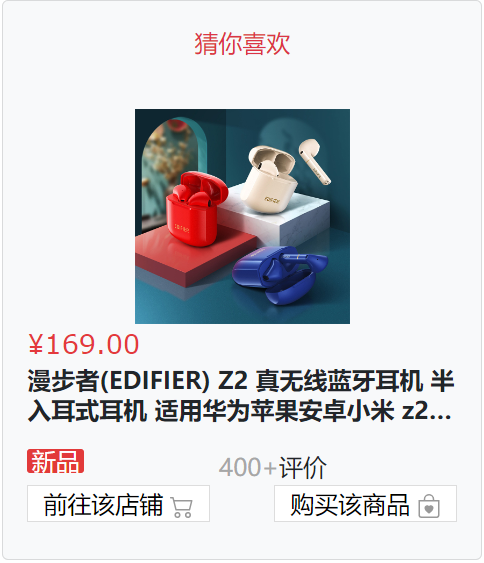
\includegraphics[scale=0.7]{pic/pic2.png}
        \caption{优化后的商品展示模块效果图}
        \label{fig:2}
    \end{figure}

    从图中可以看出,我们的商品模块主要包含以下几部分核心信息:
    \begin{itemize}
        \item 商品价格:其设计样式参考了京东商品价格的展示。利用F12定位相应的HTML元素,我们可以提取这个元素所对应的CSS属性,进而将其嵌入到网页中,其CSS样式如下
        
        \begin{lstlisting}[language=html]
    .price_font {
        color: #e4393c;
        text-align: left;
        font-weight: 400;
        font-size: large;
        font-family: Verdana;
    }
        \end{lstlisting}

        \item 商品标题:根据京东的设计理念(以及显示上的美观性),我们将标题的长度限制为两行,超出的部分以省略号替代。类似地,我们借鉴京东的字体和格式,构建了如下的CSS代码
        
        \begin{lstlisting}[language=html]
    .title_font {
        text-align: left;
        font-weight: bold;
        overflow: hidden;
        text-overflow: ellipsis;
        -webkit-line-clamp: 2;
        word-wrap: break-word;
        display: -webkit-box;
        -webkit-box-orient: vertical;
        line-height: 20px;
    }
        \end{lstlisting}

        \item 商品关键词:对于京东的产品而言,此处显示的往往是“自营”、“京东配送”;而对于我们所提取到的苏宁易购的相关产品,这里所提取的信息往往是对商品卖点或优惠政策的概括。由此,我们在此处处理为商品的“关键词”属性,并且用类似京东的红白配色予以高亮,其CSS代码如下
        
        \begin{lstlisting}[language=html]
    .goods-icons {
        float: left;
        height: 16px;
        line-height: 16px;
        padding: 0 3px;
        margin-right: 3px;
        overflow: hidden;
        text-align: center;
        font-style: normal;
        font-size: 16px;
        background: #e23a3a;
        color: #FFF;
        cursor: default;
        border-radius: 2px;
    }
        \end{lstlisting}

    \item 商品评价数:衡量产品质量以及热门度的一个非常重要的指标,在这里我们同样用类似京东的配色和现实方式来提供最为直观的体验,其CSS样式如下
    
    \begin{lstlisting}[language=html]
    .number_comments {
        color: #a7a7a7;
        font-weight: 400;
    }
    \end{lstlisting}

    \item 店铺链接和商品链接:作为电商产品的一个检索库,提供所展示商品的链接信息是十分必要的。在这里我们还使用了Bootstrap所提供的矢量Icon来辅助美化,起到了不错的效果。链接的到的网址通过flask框架接入HTML的href属性,而小标签的插入则利用svg标签来进行。
    
    由此,我们也就构建了较为清晰整洁的商品展示块(Block),考虑到整体网页的设计,我们令一页最多展示15行(共45个商品),并设计了分页条。由于时间的限制,我们将分页条所包含的页面数量设置成了一个定值(15),也就意味着我们最多展示15页商品(这一做法参考了亚马逊的实现)。我们小组认为,按照相关度的降序排列,15页的商品总数足以满足一般查找的需要;为了更加精细化的查找需求,我们也设计了过滤器等其它功能来进行辅助。

    对于分页条的实现,我们参考了Bootstrap中的pagination模块,并且通过细致的分支语句做到特定场景下button的灰、蓝转化,如图\ref{fig:3}、\ref{fig:4}所示。

    \begin{figure}[H]
        \begin{minipage}{0.49\textwidth}
            \centering
            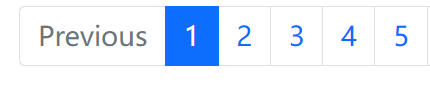
\includegraphics[scale=0.5]{pic/pic3.png}
            \caption{Page=1时的显示}
            \label{fig:3}
        \end{minipage}
        \begin{minipage}{0.49\textwidth}
            \centering
            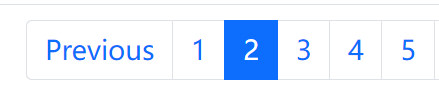
\includegraphics[scale=0.5]{pic/pic4.png}
            \caption{Page=2时的显示}
            \label{fig:4}
        \end{minipage}
    \end{figure}

    为了实现链接到不同页面的功能,我们在Flask后端加入page属性与html进行互联。我们在HTML中书写时\textbf{使用"/result?argName={{argVal}}"的方式进行传参},而利用链接进行传参后在后端使用request.args.get()方法进行提取。上述方法对应的HTML核心代码如下所示。

    \begin{lstlisting}[language=html]
    
        
        <li class="page-item active" aria-current="page">
            <a class="page-link" 
            href="/result?keyword={{keyword}}&page={{i+1}}">
            {{i+1}}</a>
        </li>
        
        <li class="page-item">
        <a class="page-link" 
        href="/result?keyword={{keyword}}&page={{i+1}}">
        {{i+1}}</a>
        </li>
        
    
    \end{lstlisting}

    在python代码中,我们需要将得到的所有搜索结果进行划分,根据提取到的关键字page的值来返回对应位置的搜索结果。在下述代码中,left\_bound和right\_bound便给出了对应的左右边界。

    \begin{lstlisting}[language=Python]
    actual_length = len(results[0])
    if actual_length % 50 != 0:
        max_page = actual_length // 50 + 1
    else:
        max_page = actual_length // 50
        
    max_page = min(max_page, 15)
    
    left_bound = int(50 * (page - 1))
    right_bound = min(int(50 * page), actual_length)
    \end{lstlisting}

    \end{itemize}
    
    

    \subsection{筛选模块的设计与实现}

    在京东的商品搜索的主界面上,含有非常丰富的筛选模块。例如对于我们所研究的“耳机”这一基本关键词,京东所给出的可细化的选项如图\ref{fig:5}所示。我们参考京东的设计对其进行了简化,主要聚焦于\textbf{品牌}和\textbf{耳机佩戴方式}这两种基本的产品属性来构建筛选体系,其可视化界面如图\ref{fig:6}所示。

    \begin{figure}[H]
        \centering
        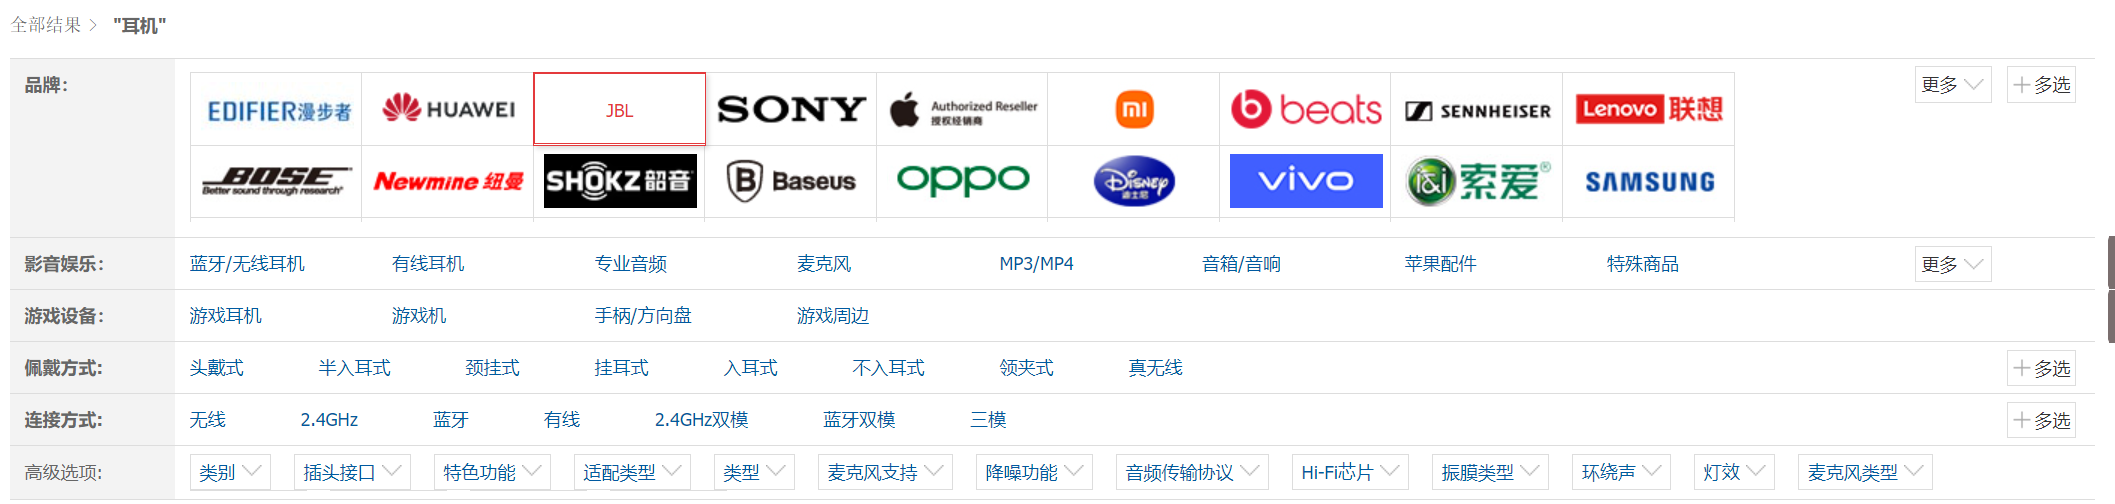
\includegraphics[scale=0.4]{pic/pic5.png}
        \caption{京东对于“耳机”这一关键词的二级筛选项}
        \label{fig:5}
    \end{figure}

    \begin{figure}[H]
        \centering
        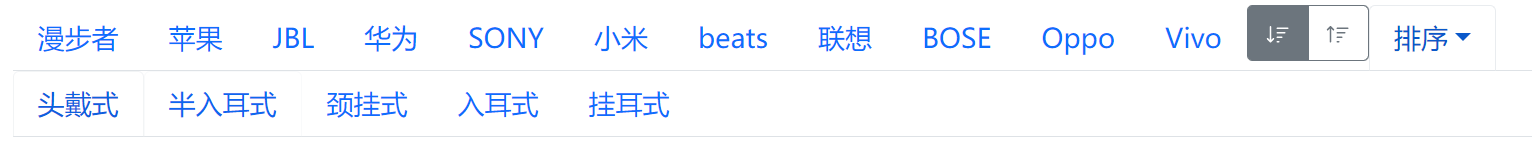
\includegraphics[scale=0.6]{pic/pic6.png}
        \caption{我们小组所设计的二级筛选项}
        \label{fig:6}
    \end{figure}

    为了能够实现筛选以及关键词拼接的功能,我们在HTML的代码中引入brand\_filter变量用于记录筛选器的种类,并且将对应的关键词与用户已经输入的关键字进行拼接,进而作为新的关键字进入后端进行新一轮的搜索,最后将得到的结果进行反馈,完成筛选过程。为了排版的规整性,我们引入BootStrap中的导航栏(nav)组件以及Container组件来进行构建,其核心的HTML代码如下

    \begin{lstlisting}[language=html]
    <ul class="nav nav-tabs">
        
        <li class="nav-item">
            <a class="nav-link" 
            href="/result?keyword=SONY {{keyword}}
            &brand_filter=1&page={{page}}">
            SONY</a>
        </li>
        ...
    </ul>
    \end{lstlisting}

    下面,我们给出筛选搜索的具体样例。图\ref{fig:7}展示了以关键词“耳机”作为关键词的搜索结果,而图\ref{fig:8}则为添加了“头戴式”这个限制条件后的搜索结果。进一步地,我们还可以在原先的基础上添加“SONY”这个筛选条件,此时我们的关键词已经变成了“耳机 头戴式 SONY”,不难看出图\ref{fig:9}所展示的结果较为符合要求。

    \begin{figure}[H]
        \centering
        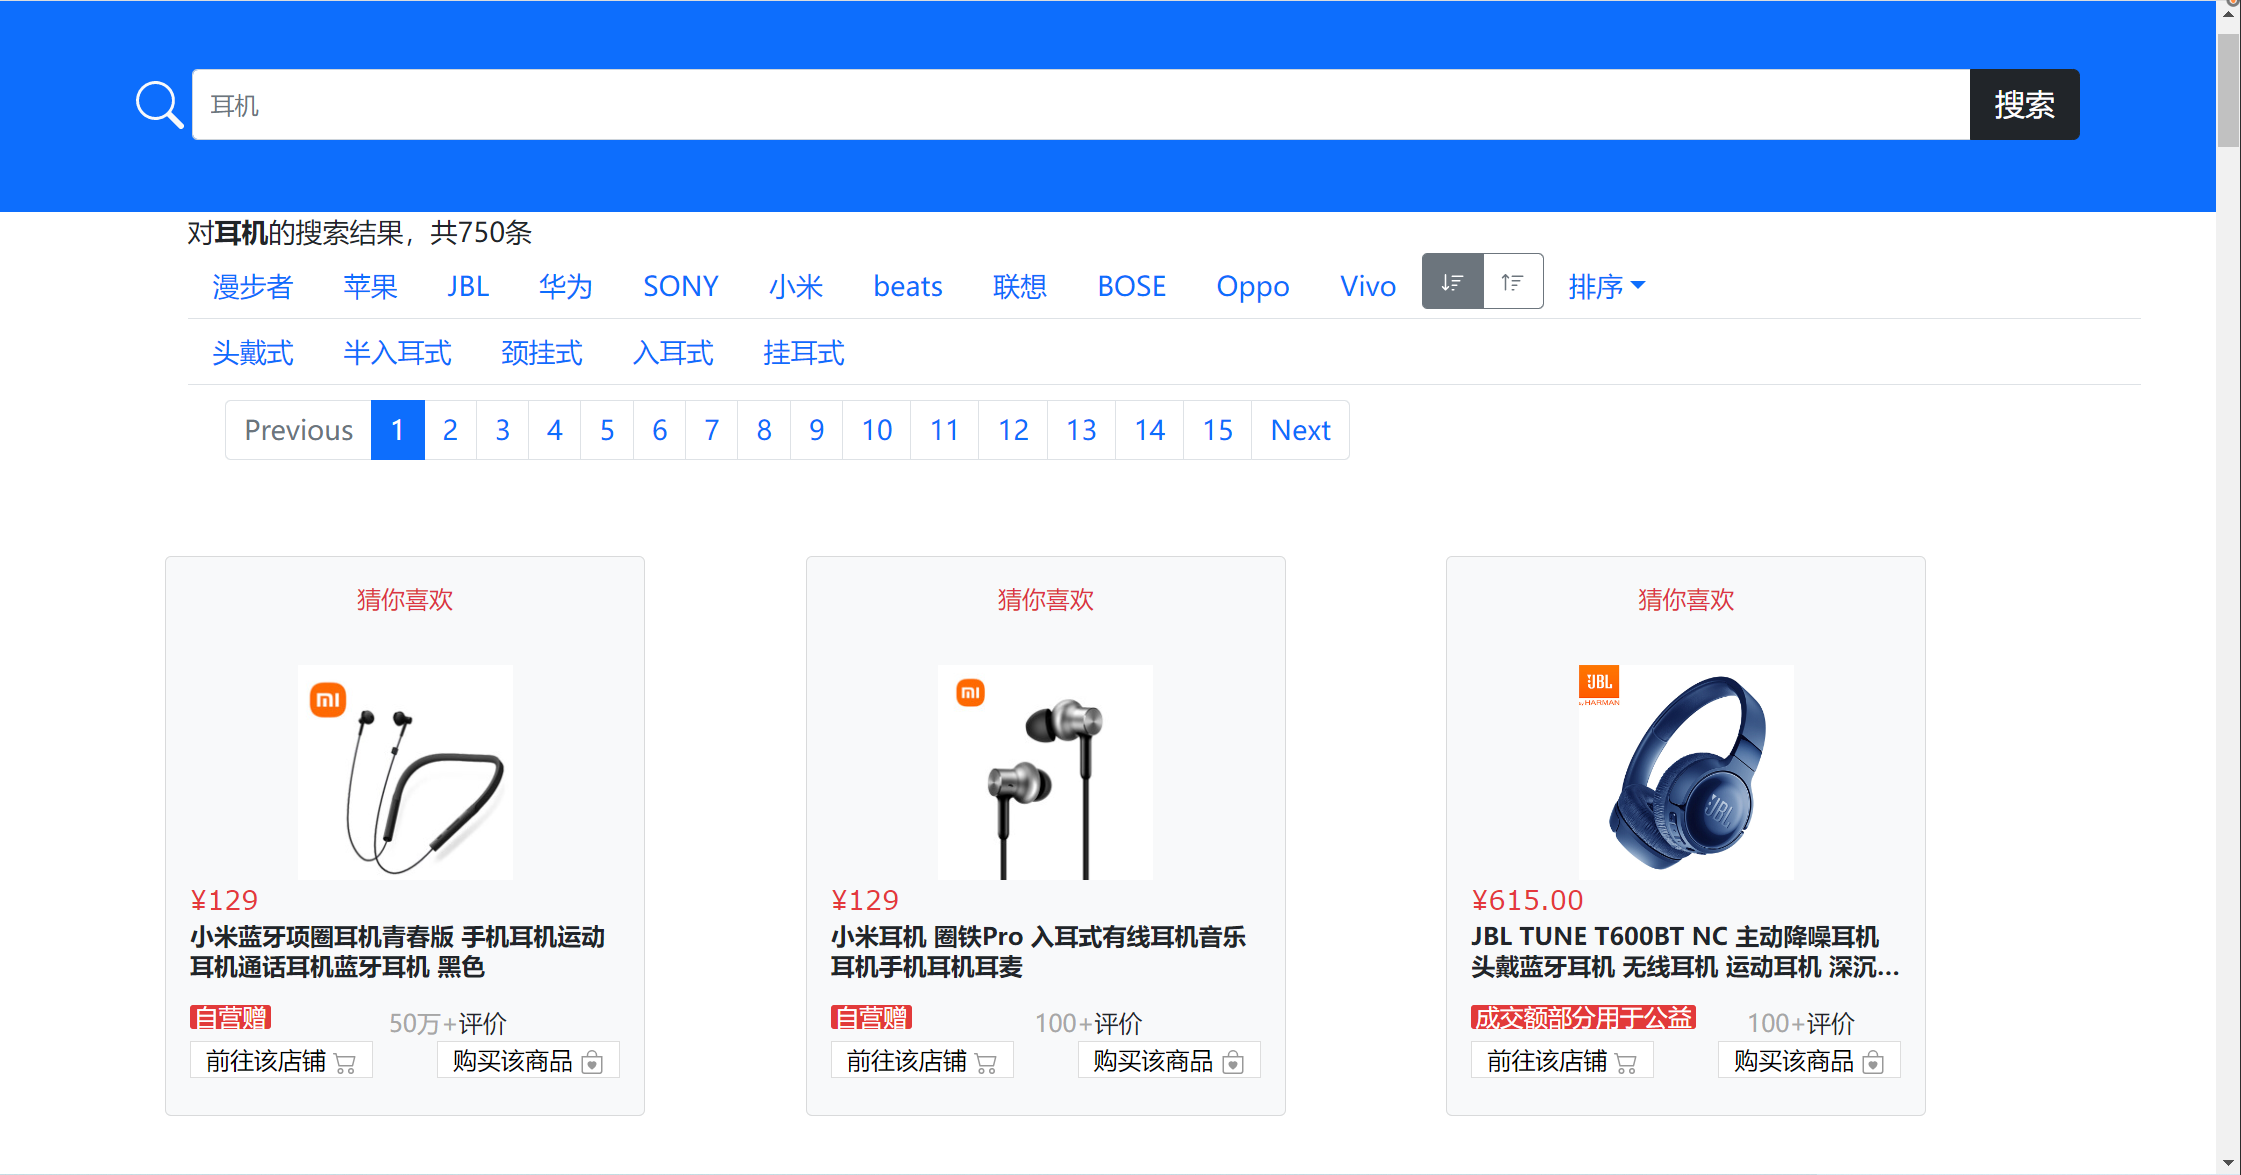
\includegraphics[scale=0.4]{pic/pic7.png}
        \caption{关键词为“耳机”所得到的结果}
        \label{fig:7}
    \end{figure}

    \begin{figure}[H]
        \centering
        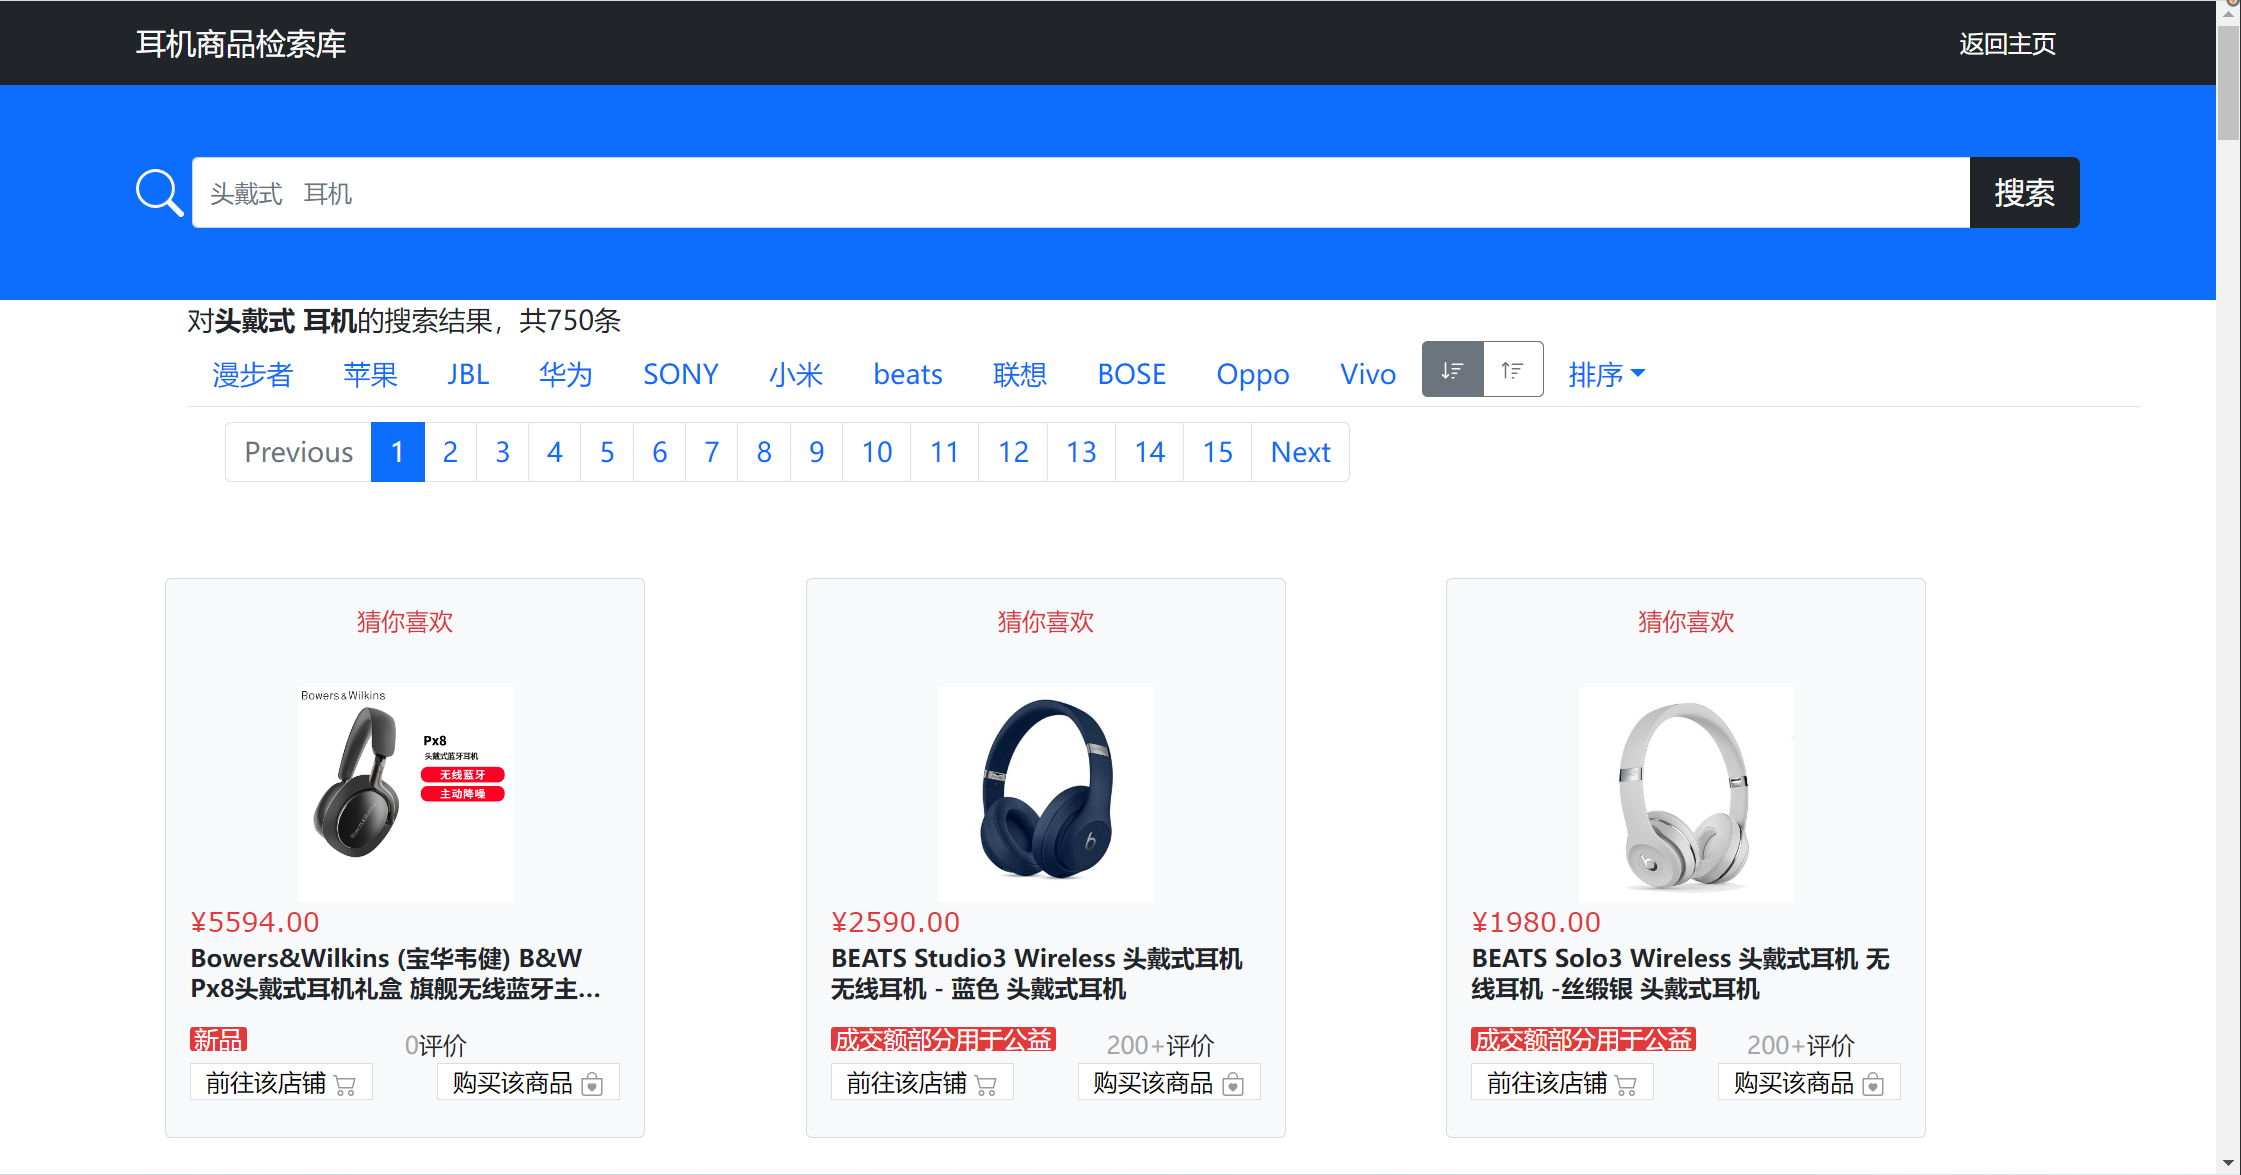
\includegraphics[scale=0.4]{pic/pic8.png}
        \caption{关键词为“头戴式\&耳机”所得到的结果}
        \label{fig:8}
    \end{figure}

    \begin{figure}[H]
        \centering
        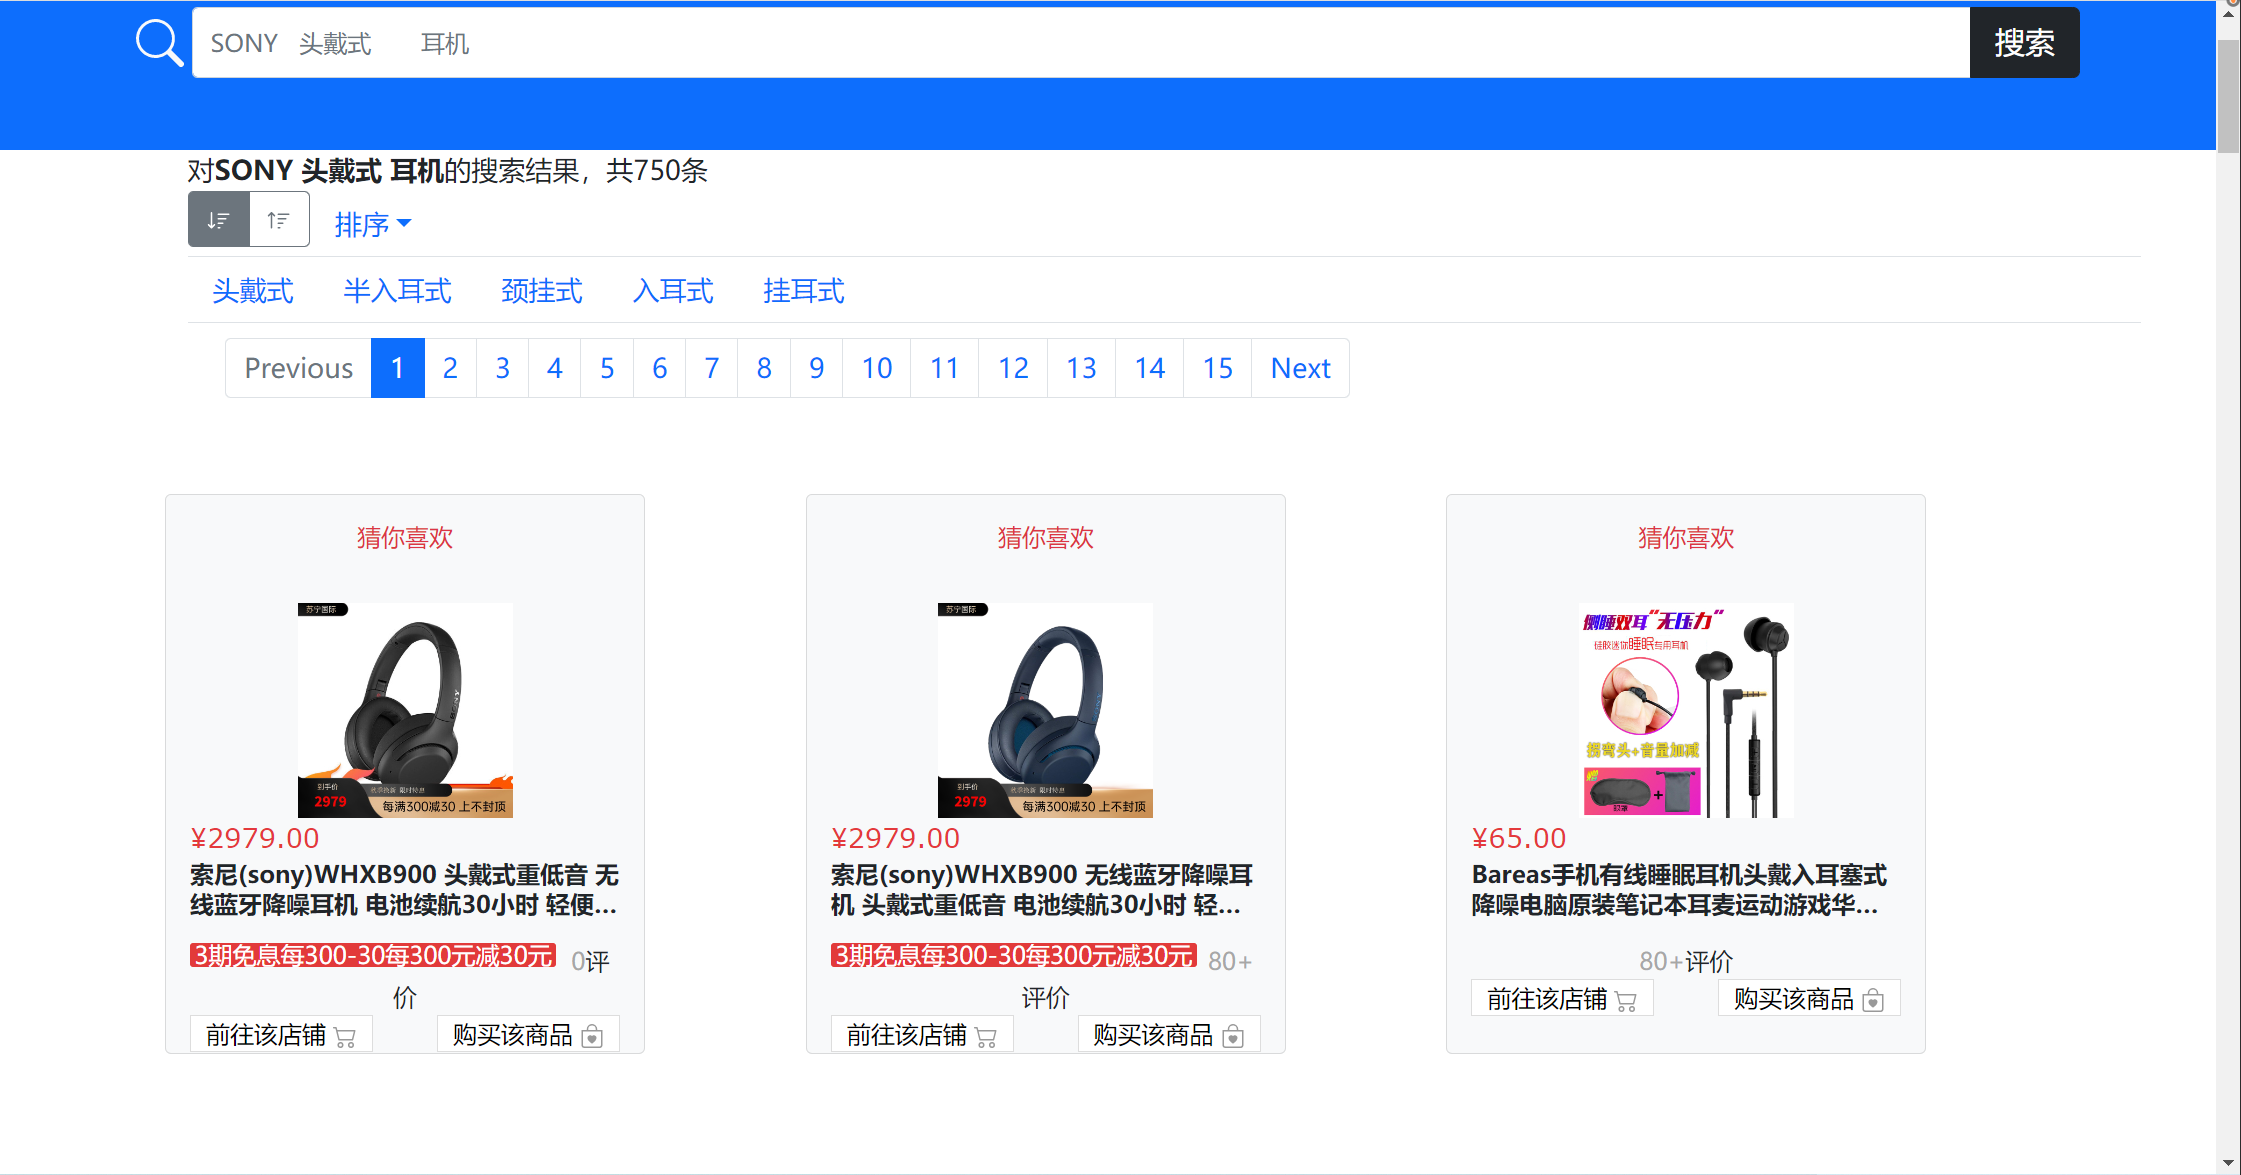
\includegraphics[scale=0.4]{pic/pic9.png}
        \caption{关键词为“SONY\&头戴式\&耳机”所得到的结果}
        \label{fig:9}
    \end{figure}

    从这三张图中还可以对比看出,当已经选中了一类的筛选标签(tag)后,再次看到该结果时这一类tag将被隐藏。但由于时间所限,借助brand\_filter这一辅助参数的思路无法应对两类标签都被选中(也即都需要隐藏)的情况,实际效果如图\ref{fig:9}所示,但并不影响整体的体验。事实上,诸如“SONY 小米”这样的结果在一些时候也可能会遇到,在我们进行实验的时候也发现部分商家会利用搜索引擎的工作原理在标题上尽可能的堆叠类似的tag,以增加自己产品所被搜索到的可能性。

    \subsection{排序模块的设计与实现}

    与筛选模块类似,排序模块同样利用前后端之间特殊参数的传递来确定当前商品展示的状态。在前文中已经给出了京东的几种典型的排序依据,在这里我们主要采用三种排序方式:相关度、价格以及商品评论。

    在讨论其工程实践之前,首先给出相关度排序方法的理论依据。在Lab 6中,我们集中讨论了各种相似性度量函数对于搜索结果的影响,而在这里我们便采用了lucene内置函数所使用的BM25相似性判定法。其基本原理如下:BM25算法将输入的句子sentence进行分词(前文已经提过,我们采用了jieba分词和lucene所提供的WhitespaceAnalyzer的结合来处理中文文本),然后分别计算句子中每个词$q$与文档$d$的相关度,然后进行加权求和。得到句子与文档的相关度评分。评分公式如下:
    \begin{equation}
        \text{Score}(Q,d, D)=\sum\limits_i^n W_iR(q_i, d)
    \end{equation}
            
    其中$W_i$为权重,即TF-IDF算法中的IDF值,$R(q_i, d)$则是$q_i$与文档$d$的相关度。IDF是用于惩罚文本中出现频数较高的词所引入的量(例如在中文文本中“这”、“了”等词语出现的次数较高,但并没有实际意义),其原始表达形式如下:
    \begin{equation}
        \text{IDF}(q_i, D)=\log \frac{N}{n_i}
    \end{equation}
    
    其中$N$为表示语料库$D$中文档的总数,而$n_i|\{d\in D, q_i\in d\}|$表示语料库$d$中含关键词$q_i$的文件数目。在lucene中,采用了这一公式的一个简单变体:
    \begin{equation}
        \text{IDF}(q_i, D)=\log \frac{N-n_i+0.5}{n_i+0.5}
    \end{equation}
    
    而上文所使用的相关系数,则可以通过如下方式来进行计算:
    \begin{equation}
        R(q_i, d)=\frac{f_i(k_1+1)}{f_i+K}\cdot \frac{qf_i(k_2+1)}{qf_i+k_2}
    \end{equation}
    
    \begin{equation}
        K=k_1(1-b+b\cdot \frac{l_d}{\text{avg }l_d})
    \end{equation}
    
    在两式中,$k_1, k_2, b$为调节因子,一般根据经验取$k_1=2$,$b=0.75$;$f_i$表示$q_i$在文档$d$中出现的频率,$qf_i$为$q_i$在输入句子中的频率。$l_d$为文档$d$的长度,$\text{avg }l_d$为文档$D$中所有文档的平均长度。又因为在绝大部分情况下,$q_i$在句中只出现一次,即所有的$q_i$的$qf_i$基本相同,因此我们可以将$k_2$取0,然后将上述公式进行简化,即省去公式的右半部分。我们不难发现,在计算相关系数的时候,同时考虑了TF(term frequency)和单个句中的词频,是对课堂中所提到的TF-IDF的一种优化。

    基于上述的理论依据,lucene所给出的similarity评分自然可以作为相关度的大小依据。以相关性作为排序属性对搜索到的商品降序排列也就成为了本搜索引擎中的默认排序规则。针对价格排序,也是建立在商品相关系数大于某个特定值时才予以进行。事实上,我们只考虑相关系数位于前15页的商品,也只对这些商品进行排序;其余搜索得到的商品由于相关性不足而不参加基于价格或者评论的排序。

    为了实现前端与后端的数据交互,我们引入sort这一变量来记录当前的排序方式。之后,在python中编写相应的代码来依照不同的属性来进行进一步的处理和排序,也就得到了如下所示的代码。

    \begin{lstlisting}[language=python]
    def sort_(result, method, reverse_opt):
        products = []
        for i in range(len(result[0])):
            product = []
            for j in range(10):
                product.append(result[j][i])
            products.append(product)
        if method == "price":
            products = product_price_processing(products)
        elif method == "quality":
            products = comments_num_sort(products)
            products = comments_num_string(products)
        results = [[] for _ in range(10)]
        for each in products:
            for i in range(10):
                results[i].append(each[i])        
        if reverse_opt == 1:
            results = reverse_(results)
        return results
    \end{lstlisting}

    为了用户使用的方便,我们还引入了\textbf{正序/逆序}的选择,通过维护reverse变量来进行参数传递。在图\ref{fig:10}中展示了商品排序的可视化界面。

    \begin{figure}[H]
        \centering
        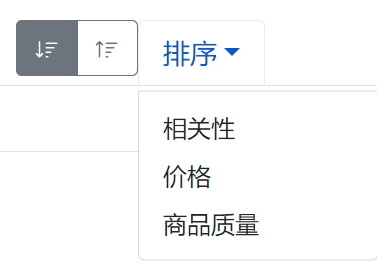
\includegraphics[scale=0.5]{pic/pic10.png}
        \caption{商品排序的功能界面}
        \label{fig:10}
    \end{figure}

    针对价格的排序相对比较好处理,考虑到有些商品并没有提供价格(例如京东商城中对于某些商品会显示“暂无价格”),我们在排序时认为这些商品的价格为0来进行操作。相关操作的代码展示如下,而图\ref{fig:11}、\ref{fig:12}则作为样例展示了关键词为“JBL”时按商品价格升序/降序排列时的结果。在图\ref{fig:12}中还可以看出一个细节:收集到的数据中有些商品并没有图片,因而我们采用Bootstrap中所提供的图标来进行代替,这样能够保证排版的统一性。

    \begin{figure}[H]
        \centering
        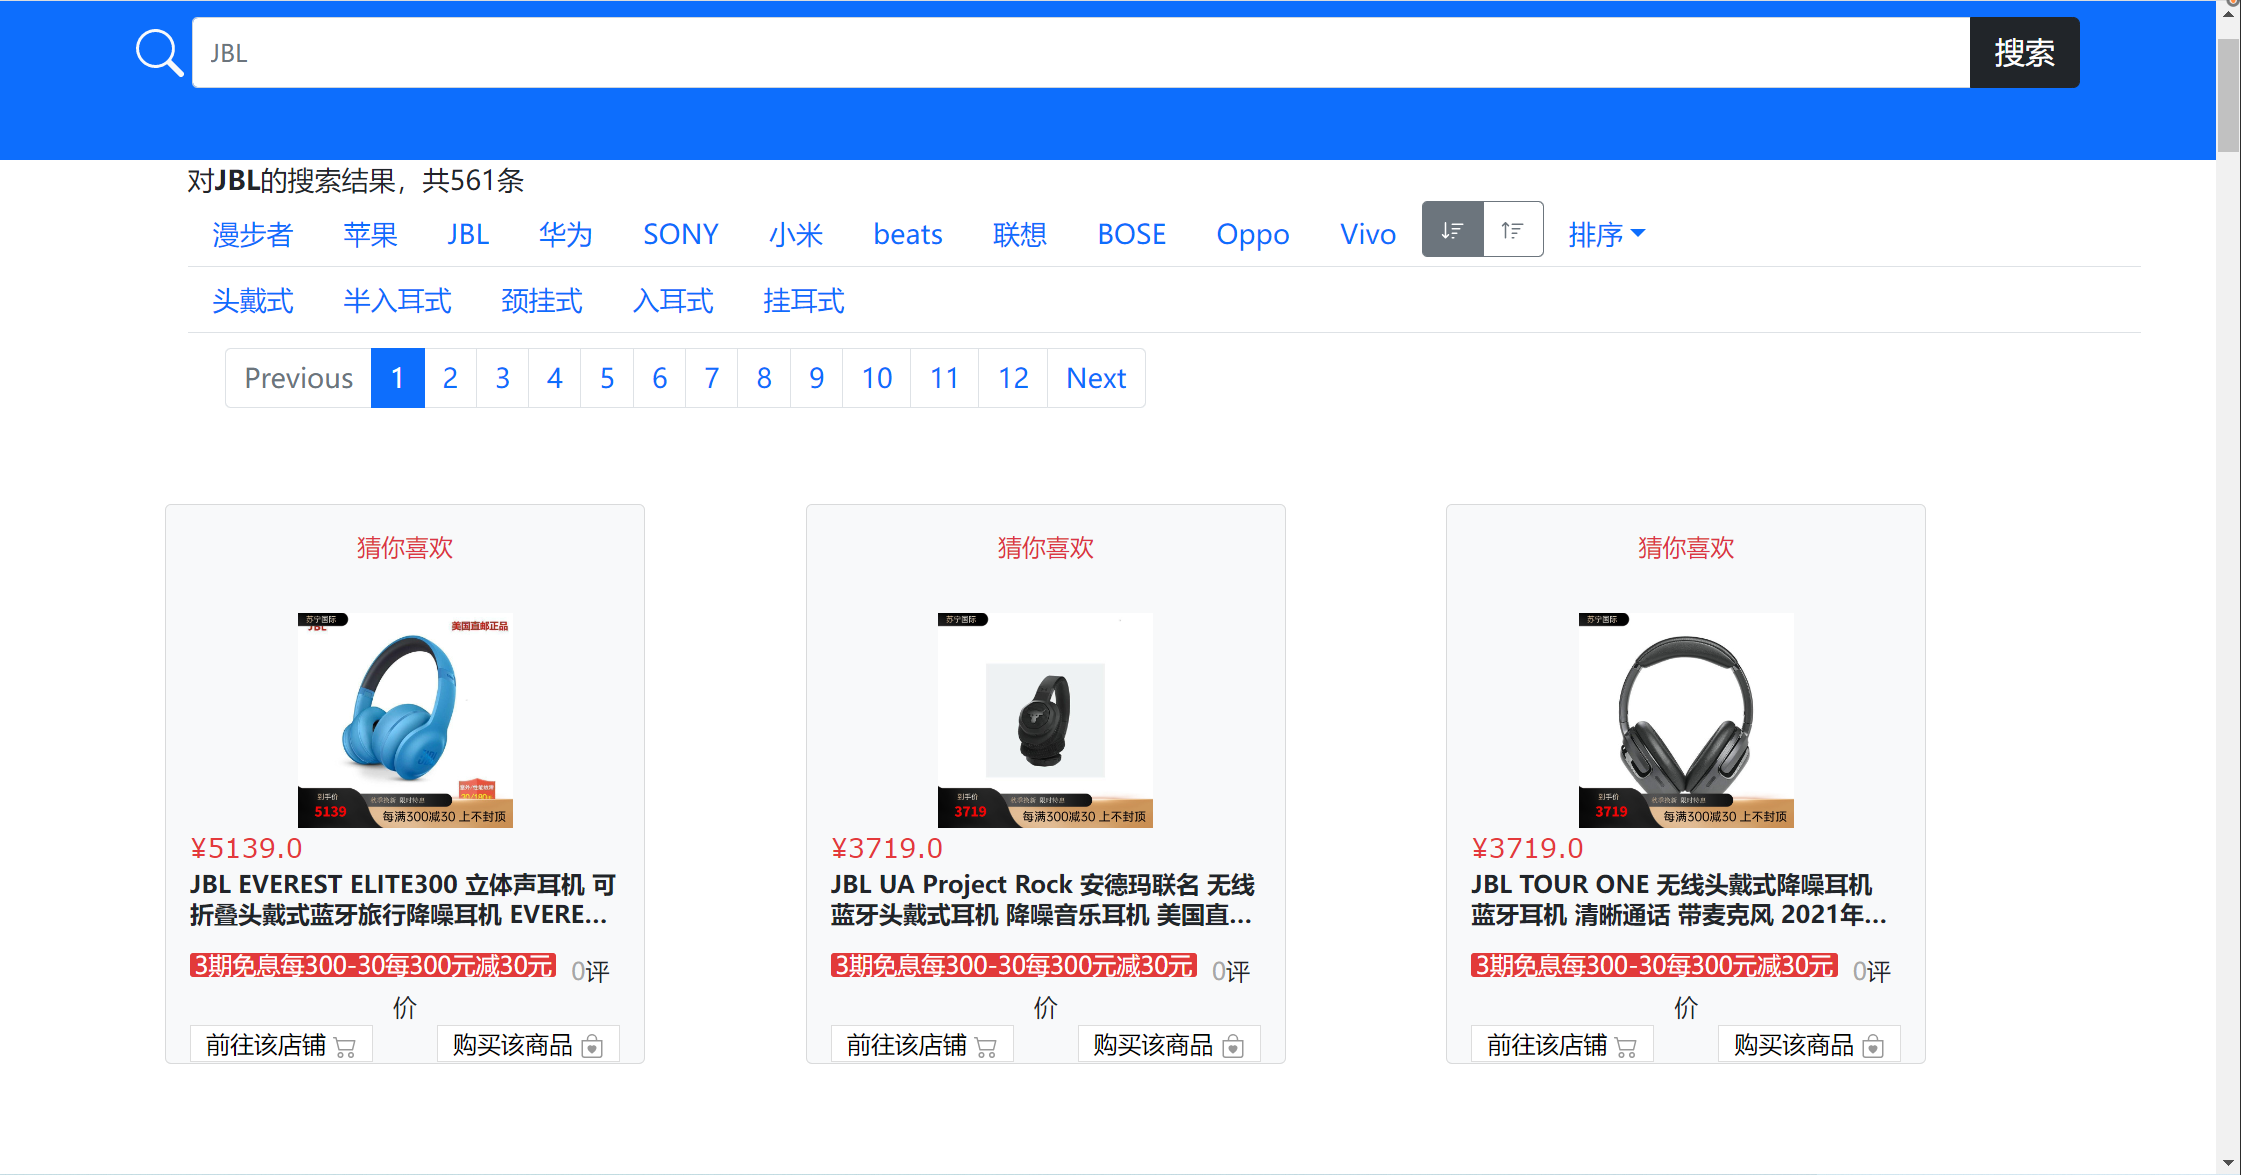
\includegraphics[scale=0.4]{pic/pic11.png}
        \caption{关键词为“JBL”、按商品价格降序排列}
        \label{fig:11}
    \end{figure}

    \begin{figure}[H]
        \centering
        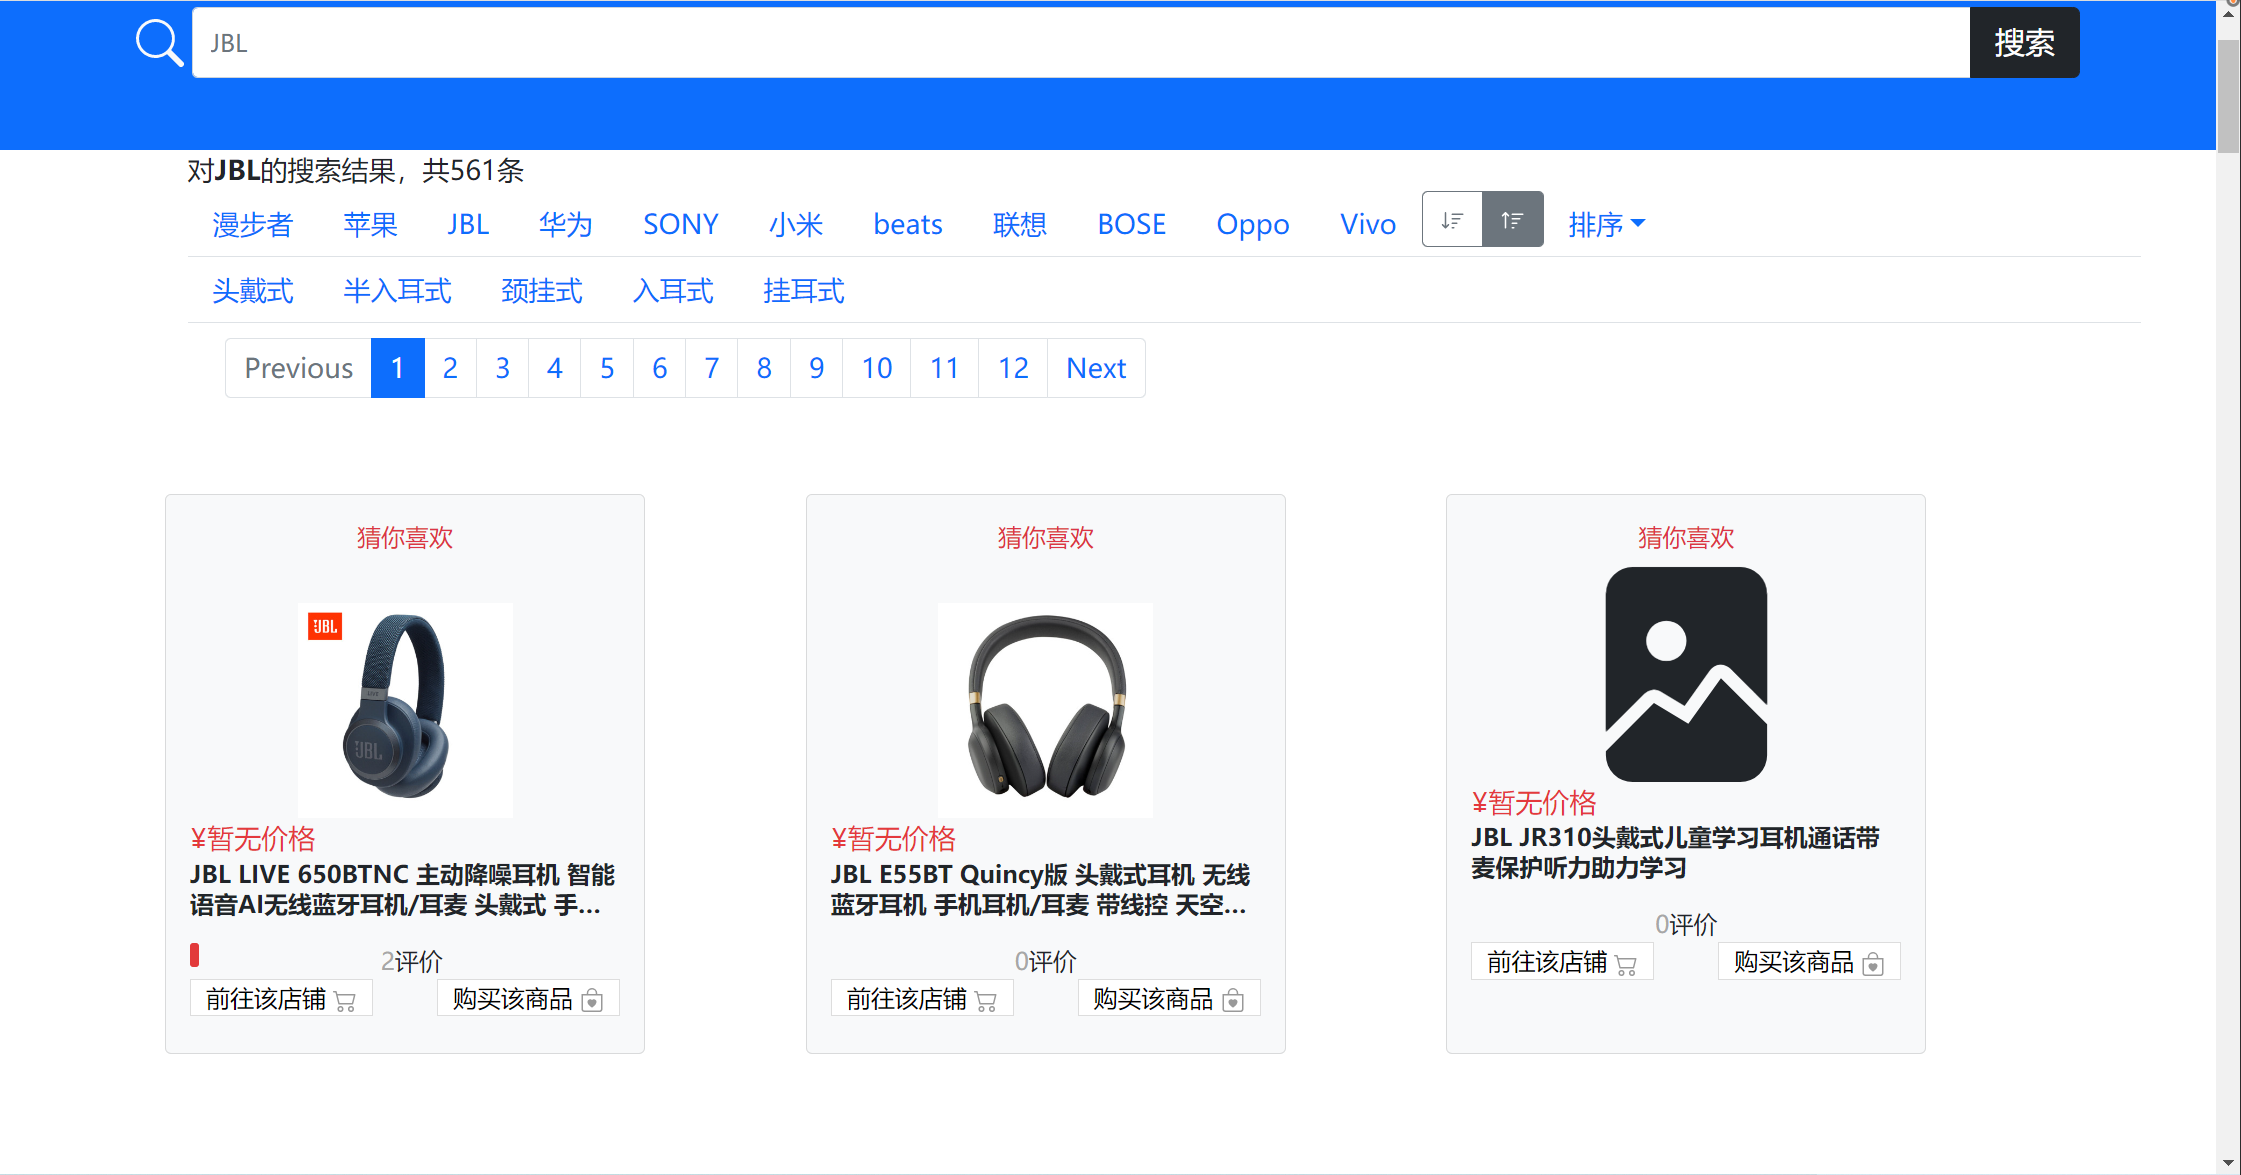
\includegraphics[scale=0.4]{pic/pic12.png}
        \caption{关键词为“JBL”、按商品价格升序排列}
        \label{fig:12}
    \end{figure}

    最后,我们考察基于商品评论的排序。本次大作业的一个选做项的要求为“基于产品的评论来对产品质量进行估计”,并根据估计的结果来进行排序。但考虑到运行速度的限制,对于每一个可能的搜索结果再进一步爬取其对应的评论,利用LDA等方法进行情感分析,进而返回相应的结果过于繁琐。事实上,在美国大学生数学竞赛(MCM)2020年的C题中,就给出了一个类似的样例:针对Amazon所提供的五种产品以及五种产品所对应的上万条评论,要求进行一系列分析。由于时间有限且爬虫水平受限,对于二级信息的爬取受到京东反爬机制的限制,因而我们退而求其次选择了\textbf{基于商品评论数的排序}。其基本代码实现如下

    \begin{lstlisting}[language=python]
    def comments_num_sort(products):
        for i in range(len(products)):
            flag = False
            if "WAN" in str(products[i][5]):
                flag = True
            products[i][5] = int(float("".join(list(filter(lambda x: str.isdigit(x) \
            or x==".", list(str(products[i][5])))))))
            products[i][5] *= 10000 if flag else 1            
            
        products.sort(key=lambda x: int(x[5]), reverse=True)
    return products
    \end{lstlisting}

    基于商品评论数的排序所得到结果如图\ref{fig:14}所示,符合预期。事实上,在京东的网上商城中,同样拥有类似的“评论数”排序的选项。

    \begin{figure}[H]
        \centering
        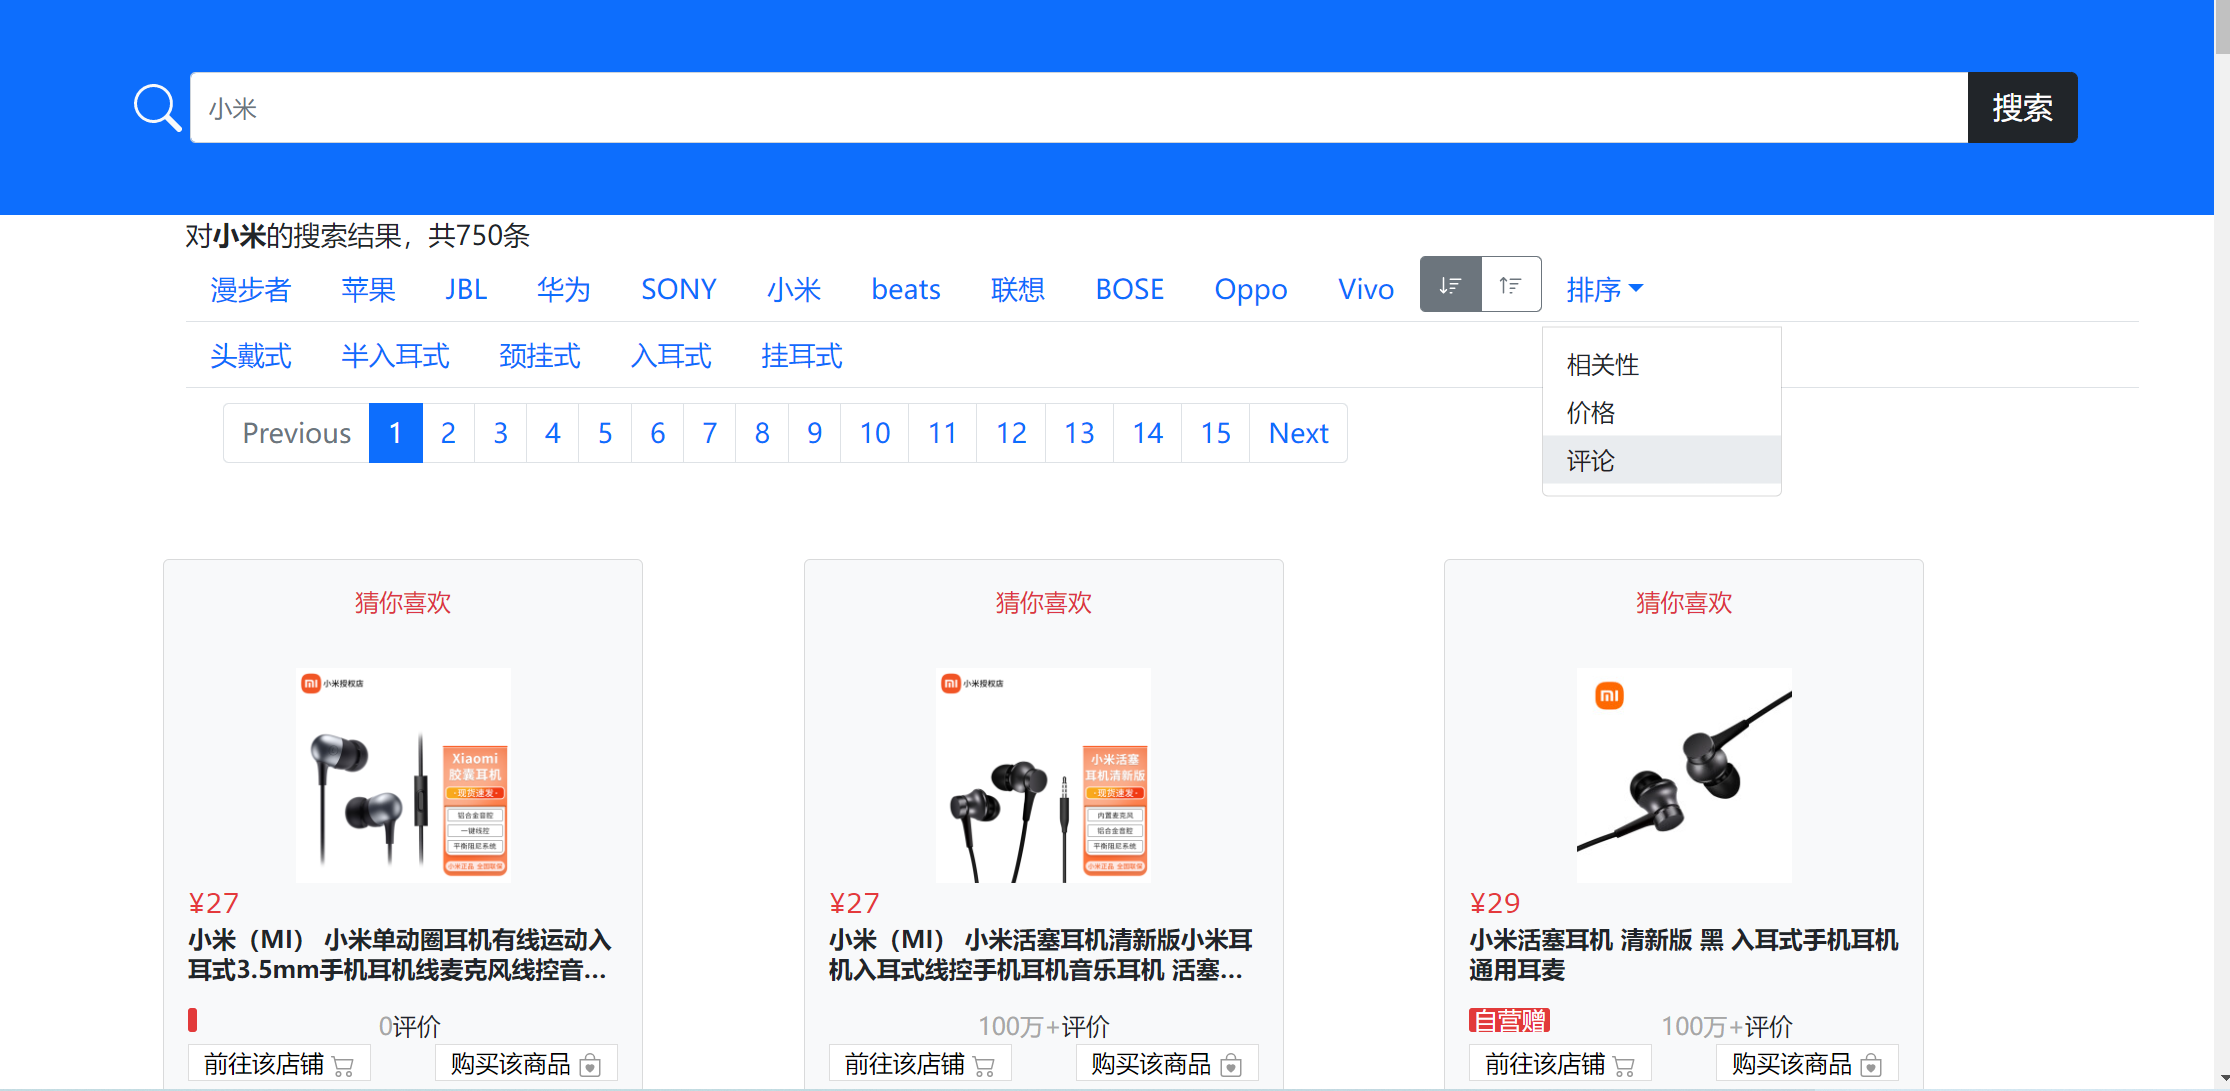
\includegraphics[scale=0.4]{pic/pic14.png}
        \caption{关键词为“头戴式\&小米”,按评论数降序排列}
        \label{fig:14}
    \end{figure}
    





    \section{基于神经网络的图片识别算法}

    \section{总结与拓展思考}

    

\end{document}